% Syslab Research Journal Template
% By Patrick White
% September 2019

% Do not edit this header
\documentclass[letterpaper,11pt]{article}
\usepackage{fullpage}
\usepackage{palatino}
\usepackage{enumitem}
\usepackage{courier}
\usepackage{graphicx}
\def\hrulefill{\leavevmode\leaders\hrule height 20pt\hfill\kern\z@}

% ------------- Edit these definitions ---------------------
\def\name{Bryan Lu}
\def\journalnum{15}
\def\daterange{01/20/20-02/10/20} % starts on Monday
\def\period{2}
% ------------------ END ---------------------------------
% Do not edit this
\begin{document}
	\thispagestyle{empty}
	\begin{flushright}
		{\Large Journal Report \journalnum} \\
		\daterange\\
		\name \\
		Computer Systems Research Lab \\
		Period \period, White
		\end{flushright}
	\hrule height 1pt

% ------ SECTION DAILY LOG -------------------------------------
\vspace{-0.8em}
\section*{Daily Log}
%Detail for each day about what you research, coded, debug, designed, created, etc. Informal style is OK.
\vspace{-0.8em}

\subsection*{Tuesday, January 21}
\vspace{-0.6em}
Tried running the same sentence with all of the different options that the Stanford parser provided in order to figure out what exactly was being parsed by the code in the next lines. 

\vspace{-1.3em}
\subsection*{Thursday, January 23}
\vspace{-0.6em}
Gave up on hoping one of the parsing methods was just going to give the answer outright, started looking into the structure of the parsing of the dependency tree to start altering the method itself. Sent another email requesting status update on annotations. 
\vspace{-1.3em}
\subsection*{Wednesday, January 29}
\vspace{-0.6em}
Continued debugging and rewriting the dependency tree parsing, and provided fixes to errors as they arose. 
\vspace{-1.3em}
\subsection*{Thursday, January 30}
\vspace{-0.6em}
Finished rewriting dependency tree parsing, got syntax parsing code to run all the way through for a test case, and also successfully ran the syntax parsing on an olympiad problem. 
\vspace{-1.3em}
\subsection*{Monday, February 3; Tuesday, February 4}
\vspace{-0.6em}
Worked on and prepared for presentation, and watched presentations in class. 
\vspace{-1.3em}
\subsection*{Thursday, February 6}
\vspace{-0.6em}
Skimmed through annotation data found under ``Issues'' tab on original project github page, and began trying to parse it and matching it up against test cases, while also paying attention to presentations. 
\vspace{-0.8em}

% ------ SECTION TIMELINE -------------------------------------
%\newpage
%\vspace{-1.7em}
\vspace{-1.0em}
\section*{Timeline}
\begin{tabular}{|p{1in}|p{2.5in}|p{2.5in}|}
	\hline
\textbf{Date} & \textbf{Goal} & \textbf{Met}\\ \hline 
	\hline
1/20 & Adapt the question input for their code to access local files instead of a database, try running their code with olympiad problems. & I didn't get this done, but I can get away with pushing this to next week as I still don't have annotation data to play with yet. \\
	\hline 
1/27 & Pending annotations, get everything up until the annotations step to work with olympiad problems, and work out other cosmetic details. & Yes! My snippet can output syntax parses for individual problems now, but I won't do local problem access until I have to run it multiple times with the tag model. \\
	\hline
2/3 & Assuming I have annotation data, run it through the parser to check it works, and format olympiad problems in that method. Else, begin trial and error process. & Couldn't do a lot of this because of presentations, but I will do this starting next week and into the week after. \\
	\hline
\end{tabular}

\begin{tabular}{|p{1in}|p{2.5in}|p{2.5in}|}
	\hline 
2/10 & Run annotation data combined with problems through code and turn them into semantic trees, reformat my annotated problems. & N/A \\
	\hline
2/17 & Finalize annotation data for the olympiad problems and ensure that they produce valid, connected semantic trees. & N/A \\
	\hline 
\end{tabular}

% ------ SECTION REFLECTION  ---------------------------------
\section*{Reflection}
%In narrative style, talk about your work this week. Successes, failures, changes to timeline, goals. This should also include concrete data, e.g. snippets of code, screenshots, output, analysis, graphs, etc.

The week of the 21st, I wasn't too productive in continuing to fix my own code snippet, considering a lot of my time was spent waiting for the Stanford parser to run (and sometimes hanging if my request was too complex and required a lot of other libraries). I looked back in the paper on Thursday and realized if the purpose of the Stanford parser was to make the dependency tree, I should maybe try to modify their code to actually do that through any means necessary instead of guessing it was something else. 

This is something I ended up doing the following week, and the code seems like it outputs a full ``syntax parse'' for a test case, shown below. It also works for an olympiad problem that I fed it! This is something best shown in person because it requires going into the debugger to show it works, but here's an image of an output for an olympiad problem: 
% images
\begin{center}
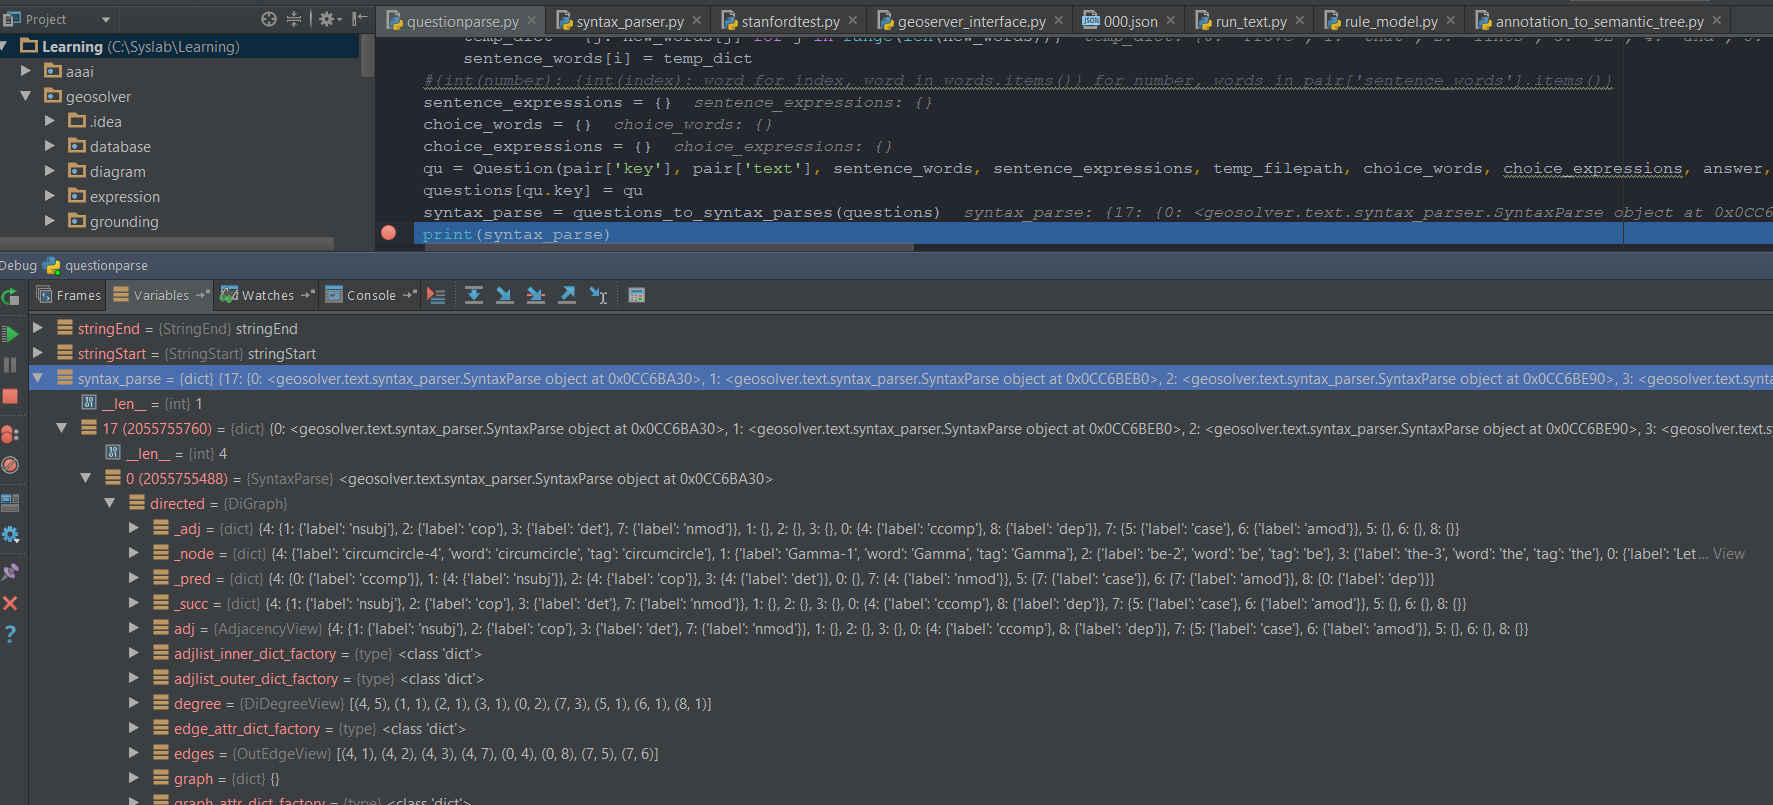
\includegraphics[scale=0.3]{syntaxparse.png}\\
\end{center}

I've asked the original author multiple times for annotation data, but I've ended up not needing his guidance anymore, because of something I found last week. Someone asked a question under the ``Issues'' tab and when I downloaded their data, it turned out to have a lot of annotations and their corresponding problems! Here is a set of annotations that I've isolated corresponding to a sentence: 
\begin{center}
sentence: In the figure above, lines AB, CD, and EF intersect at P. 

annotations: IsLine@5(line@6), IsLine@8(line@9), IsLine@12(line@13), CC@11(line@6, line@9), CC@11(line@6, line@13), IntersectAt@14(line@6, point@16)
\end{center}
The "@x"s are presumably placeholders for words that in the sentence, i.e. the explicit variable names. 
I will study these going into next week and the week after, after which I'll have everything I think I'll need to begin training for real this time. 

\end{document}

